%!TEX root = ../physical-olympics-2.tex
\chapter{运动学}


\section{时空与物质}

物理学,\,从刚开始成为实验性的科学的伽利略时期开始,\,到近半个世纪年来理论物理学家对额外维度的探讨,\,都给予了\emph{时空}(spacetime)最核心的地位.\,牛顿的理论,\,分析力学,\,经典场论,\,相对论这些理论最基本的图像都是时空与\emph{物质}(matter)的分立性.\,时空是装备了一个能体现出物理物理意义的\emph{度量}(metric)的3+1维对象\footnote{数学上有一套严格的说法,\,把这种连续,\,光滑的四维对象称为\emph{伪黎曼流形}(pseudo-Riemannian manifold).}.\,而物质是在每个时空点处的某种结构.\,下面会分别介绍不同物质体系的描述方法.\,在这之前我们来看看不同的时空观:

\subsection{时空观,\,坐标系}
牛顿力学理论体系基于\emph{伽利略时空观}(Galilean spacetime picture),\,也就是\emph{绝对时空观}(absolute spacetime picture).\,在这里空间是三维的平直空间.\,设想一个人站在该空间的某个空间点,\,他的胸前,\,头顶和右手平举的三个方向就是相互垂直的方向.\,如果以自己的臂长为标准长度,\,他能够定义空间中每两个点之间的空间间隔.\,事实上,\,这个人能够以一种正确的方式为每个空间点定义一个坐标,\,那么所有三维空间点的集合与任意两个点之间的距离为:
\[A(x,y,z)\in\mathbb{R}^3 \quad;\quad x,y,z\in\mathbb{R}\]
\[A(x_1,y_1,z_1)\;,\;B(x_2,y_2,z_2)\;:\;l^2=\overline{AB}^2=(x_1-x_2)^2+(y_1-y_2)^2+(z_1-z_2)^2\]

因为空间不同于时间,\,我们为以上数字赋予特殊的物理含义,\,也就是加上\emph{量纲}(dimension).\,如果两点坐标为$(0,0,0)$和$(1,1,1)$,\,那么$l=\sqrt{3}{\rm m}$,\,而不是$l=\sqrt{3}$.\,其单位${\rm m}$一方面表示了这个物理量的属性,\,另一方面指定了某个实际物理体系确定下来的固有长度大小.\,现行的(2018年1月1日,\,下文同)国际单位制对$1{\rm m}$的定义如下\footnote{一方面,\,它依赖于狭义相对论的正确性,\,目前极少理论物理工作者会质疑它.\,另一方面,\,应该要先定义下文的1s,\,再来定义1m.}:
\begin{verse}
1m是光在1/299792458\,s内在真空中行进的距离.
\end{verse}


这就是我们的\emph{三维平直空间}(3-dimensional flat space).\,注意空间点具有物理实际意义,\,它可以脱离坐标系而单独存在.\,事实上坐标系的原点可以建立在空间中的任意点处,\,朝向也可以是任意方向,\,两个空间点之间的距离$l$不会依赖于坐标系的选取,\,但两个点的坐标会因坐标系不同而改变.\,如果我们选取的坐标系总是下述使得两个相距很近的点之间的微元距离公式成立:
\[\ud l^2=\ud x^2+\ud y^2+\ud z^2\]


那么建立的坐标系就是一个\emph{笛卡尔坐标系}(Cartesian coordinate system),\,即\emph{空间直角坐标系}(3D orthogonal coordinate system).\,但是以空间直角坐标系为基础,\,我们又经常建立\emph{球坐标}(spherical coordinate)和\emph{柱坐标}(cylindrical coordinate)系统.\,通常取$x$轴为\emph{幅轴}(azimuth axis),\,点在$x-y$平面上的投影与原点的连线相对$x$轴转过的角度为$\varphi$,\,即\emph{幅角}(azimuth angle).\,而$z$轴为\emph{极轴}(polar axis),\,而点与原点连线与极轴的夹角$\theta$为\emph{极角}(polar angle).\,天文观测用球坐标就很方便,\,它是以描述的空间点到原点之间的距离$r$,\,也称\emph{矢径}(radius),\,和两个描述角位置的极角幅角来构成三个坐标$(r,\theta,\varphi)$的.\,而理论物理里也常用到的柱坐标是以$(\rho,\varphi,z)$为描述空间点的坐标,\,$\rho$是空间点到$z$轴的距离.

\begin{wrapfigure}[14]{o}[-10pt]{7cm}
\vspace{-0.4cm}
\centering
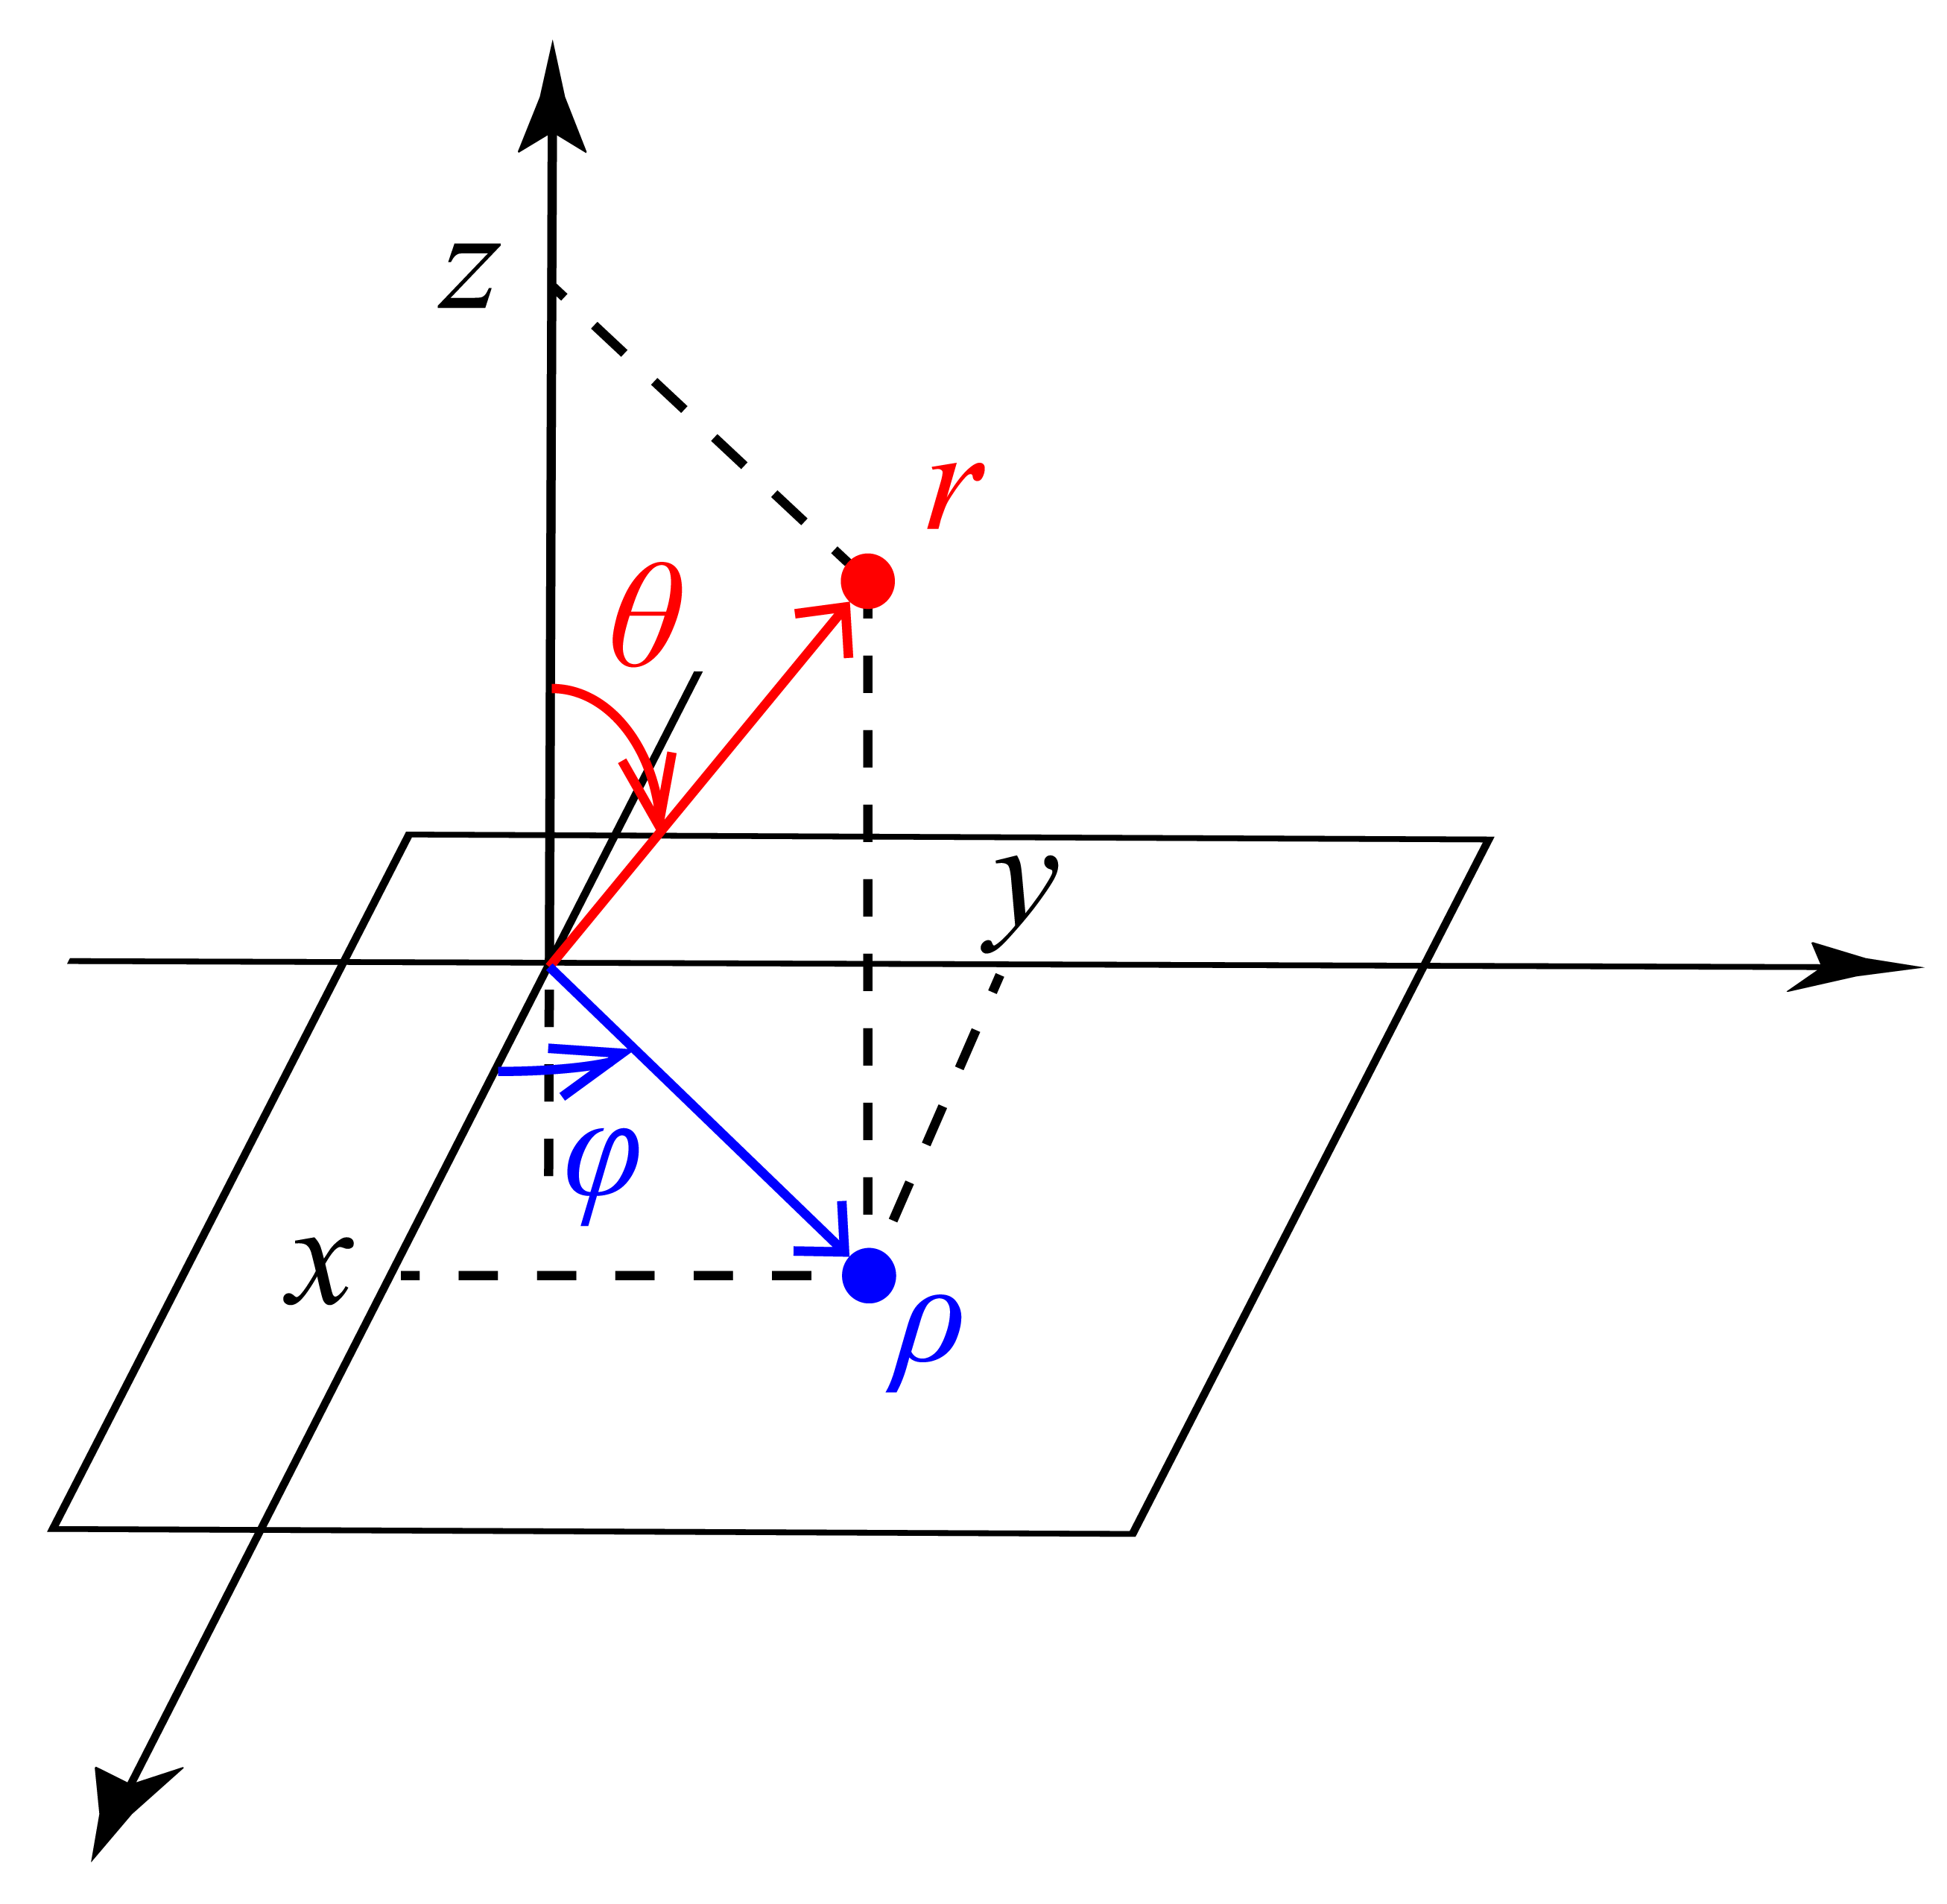
\includegraphics[width=7cm]{image/6-1-1.png}
\caption{三种坐标}
\end{wrapfigure}
需要注意,\,我们对以上$\theta,\,\varphi$角度定义比较微妙,\,$\theta$一般限制其在$[0,\pi]$范围内,\,在端点$\theta=0,\,\pi$处$\varphi$的不同取值代表同一个空间点.\,但$\varphi$的取值我们不加以任何限制,\,也就是原则上$\varphi\in\mathbb{R}$.\,而任意$\varphi$相差$2n\pi$的坐标实际上代表同一个空间点.\,这么做是因为我们最好不要用静态的几何观点去看待角度这一概念.\,而是用运动,\,变换的观点去看待角度.\,作为连续的运动的点的幅角变化也应是连续的,\,为了使点绕$z$轴一圈后幅角不至于突然改变,\,就必须默认每一点的幅角可以有多种取值,\,在具体的运动中应该灵活选择其具体取值大小.

之后经常会说到各种对称性,\,在本系列教材中我们采取如下说法:\,\emph{球对称}(spherical symmetric)仅仅代表某个函数$f(r,\theta,\varphi)$与$\varphi$无关.\,而\emph{柱对称}(cylindrical symmetric)代表的是$f(\rho,\varphi,z)$与$z$无关.\,与$\varphi$和$\theta$都无关的$f(r,\theta,\varphi)=f(r,\forall\theta,\forall\varphi)$被称为\emph{各向同性}(isotropic).\,最后\emph{中心对称}(centrosymmetric)是一个很弱的对称性,\,它仅仅代表函数在\emph{中心反演}(space inversion)下的对称性:
\[f(x,y,z)=f(-x,-y,-z)\]

绝对时空观中的时间则是一种完全与空间独立的属性.\,实际上,\,每一个空间点处的人都能感受到时间的流逝.\,十分抽象的把这些不同的时刻画在一根时间轴上,\,便是一维的时间坐标:
\[A(t)\in\mathbb{R} \quad;\quad t\in\mathbb{R}\]

而时空又是两个独立的概念.\,任意一个坐标点处都有时间轴,\,而任意一个时刻都有一个三维空间切片.\,事实上,\,我们的时空是一个3+1维的结构,\,合理地选取坐标后,\,实际上可以把时空结构写成四维坐标:
\[A(x,y,z,t)\in\mathbb{R}^4 \quad;\quad x,y,z,t\in\mathbb{R}\]

而对于任意两个时空点,\,存在绝对的时间,\,也就是可以找到两个事件的绝对时间差:
\[\tau=|t_2-t_1|\]

但空间距离却具有相对性.\,我们要求在同一时刻的同一空间切片上定义空间的度量:
\[t_1=t_2:\quad l=\sqrt{(x_1-x_2)^2+(y_1-y_2)^2+(z_1-z_2)^2}\]

不同时刻的空间,\,被线性地组织在一起,\,保证每一刻都平直的空间既不会随时间膨胀收缩,\,也不会旋转加速.\,这种时空结构被叫做\emph{牛顿-嘉当几何}(Newton-Cartan geometry)\footnote{用更为严格的语言来说,\,我们需要一个装备了一阶形式``钟''$c_\nu$和二阶逆变半正定对称张量类空间度规$s^{\mu\nu}$的四维微分流形$\mathscr{M}$:
\[\mathscr{M}:\quad s^{\mu\nu}c_{\nu}=0\]}.

时间是一个新的量纲,\,其国际单位制对$1{\rm s}$的定义为:
\begin{verse}
1s是铯-133原子基态的两个超精细能级之间跃迁所对应的辐射周期时长的9192631770倍.
\end{verse}

牛顿-嘉当几何的显著特点是物理量的定义没有所谓的\emph{协变性}(covariance).\,固然,\,在三维空间坐标框架的旋转下,\,任何物理过程中的事件所发生的位置坐标发生旋转变换,\,而几乎所有标量(比如质量,\,能量)都不变,\,几乎所有矢量(比如动量,\,角动量)都按照类似坐标变换的法则发生变换.\,但是,\,对于更普遍的一列\emph{伽利略变换}(Galilean transformation),\,也就是相对匀速运动的参考系之间的变换,\,时空坐标的形式却不能简单地推广到能量动量角动量上.

不同于绝对时空观中时间与空间成为相互独立的量纲的特点,\,狭义相对论改变了对基本物理量的看法.\,狭义相对论把时空看成为可以相互转化的不可分割的新的3+1维整体,\,同时性已然破缺.\,两个时空点之间无法定义绝对的时间间隔.\,在\emph{相对论时空观}(relativistic spacetime picture)下,\,时间和空间可以用同一把尺子去丈量:\,这是由于光速的不变性:
\[c=299792458{\rm m/s}\]

而量出来的长度叫做\emph{时空间隔}(spacetime interval):
\[\ud s^2=c^2\ud t^2-\ud x^2-\ud y^2-\ud z^2\]

这赋予时空以截然不同的结构,\,最关键的一点是,\,时间的绝对性被取消了,\,不同事件发生时间先后的比较不总是可行,\,相对论的有限速度因果律在这里取代了经典观点的时序因果律.\,我们将在本书最后介绍相对论理论.


\subsection{物质}

时空是物理过程发生的舞台.\,那么将物质引入后舞台上所演出的便是\emph{事件}(event).\,事件这个物理概念由这样的数学工具来描述:\,它的第一个要素自然是时空坐标$(\bs{r},t)$,\,是事件在时空上的外化.\,第二个要素是事件内禀的属性.\,它取决于所引入的物质种类,\,还取决于我们所关心问题的层次.\,一般用标量,\,矢量,\,乃至张量这样的数学工具来描述它.\,举例,\,电磁场物质在经典物理中用电场磁场来描述,\,但在\emph{量子力学}(quantum mechanics,\, QM)中这不够了,\,需要用矢势和标势来描述才是完整的.\,在更深的\emph{量子场论}(quantum field theory)中甚至这也是不够的.\,还需要量子化为光子才合适.\,又比如,\,电子这个很有意思的现象,\,最简单的模型是质点模型,\,内禀的属性是质量,\,动量与能量\footnote{不要认为动量能量不是内禀的而是由时空运动所决定的,\,读者可以思考在水中一个气泡的上升,\,它为体系带来的动量方向如何?}.\,然而与电磁场的经典相互作用强度告诉我们还有一项内禀属性叫做电荷量.\,近代人们惊奇地发现原来电子还固有磁矩,\,也就是电子的自旋.\,最后狄拉克等人发展出\emph{量子电动力学}(quantum electrodynamics,\,QED),\,统一地用一个四分量的旋量波函数和它的方程中的若干参数来完整地描述所有发现的电子内禀属性.

\vspace{0.5cm}
\emph{经典物理学}\footnote{本书的经典物理学指牛顿力学,\,分析力学,\,经典电磁学,\,经典统计力学与狭义相对论的范畴.}(classical physics)中涉及到的物质主要有:

\vspace{0.2cm}
{\bf 1.\,质点(point mass,\,particle)}

不得不承认质点是牛顿力学的根基,\,一切可观的结论的出发点.\,质点所对应的事件集合为时空中的一条\emph{世界线}(world line).\,每一个时间仅仅有可能只有一个事件发生.\,实际上质点的运动用\emph{运动学方程}(kinematic equation)来描述:
\[\bs{r}=\bs{r}(t)=\left(x(t),y(t),z(t)\right)\]

而\emph{质量}(mass)是质点必要的内禀属性.\,它将作为参数出现在下一节介绍的动力学方程中.\,它反应物质受到同样大小的相互作用运动状态改变的难易程度.\,国际单位制对$1\rm kg$的定义如下:

\begin{verse}
1kg是保存在法国巴黎布勒特伊宫的国际计量局实验室的约47立方厘米立式铂铱合金小圆柱的质量.\,当然,\,处于实用考虑,\,也是很多它的官方复制体的质量.
\end{verse}

这个定义从1889年至今已经有一百多年了,\,历史远长于其他六个国际基本单位.\,2018年末将有望修改这一古老的定义方式,\,新的定义\footnote{一方面,\,它依赖于狭义相对论和量子力学的正确性,\,目前极少理论物理工作者会质疑它.\,另一方面,\,应该要先定义上文的1s和1m,\,再来定义1kg.}为:

\begin{verse}
1kg被这样定义:\,取普朗克常数的固定数值在单位$\rm kg\cdot m^2\cdot s^{-1}$下为$\rm 6.62607015\times 10^{-34}$.
\end{verse}

长度,\,时间和质量为三大力学量纲,\,量纲是物理量的属性,\,物理量的表示方法为数值加单位,\,每个量纲有自己独特的一套单位,\,不同单位间差一个纯数的倍率.\,在物理量的加减时量纲必须相同而且结果保持量纲不变.\,但不同量纲物理量可以进行乘除而生成新的量纲.\,除了简单的加减乘除的以上规则以外,\,其他特殊函数必须只能作用在无量纲的纯数上.\,这叫做\emph{量纲法则}(dimensional rules).

\vspace{0.2cm}
{\bf 2.\,质点系(particle system)}

质点系是对质点的一种自然扩展.\,讨论质点的运动时质点受到的相互作用来自何方?\,在牛顿力学的框架下必然来自施力物体.\,故把两个质点作为整个体系讨论,\,把相互作用区分为内力与外力而推广之前的结论,\,在这个过程中我们能体会到哪些结论是一脉相承的普遍规律而哪些需要重新审视与修改.\,从原理上质点系不过是多个质点同时存在的情况而已.\,而经典统计力学是这种观点的提炼与延伸,\,它着眼于一个宏观大分子数的体系的长时间平均下的行为,\,理论上常常结合概率论的做法,\,对等概率的体系代表点构成的系综做平均.\,从中提取统计力学下不平凡的物理量.

\vspace{0.2cm}
{\bf 3.\,连续介质(continuous media)}

一方面,\,连续介质是从纯粹的理论过渡到实际问题的至关重要一步.\,另一方面,\,在处理连续介质的问题中形成了场论,\,它作为了一种与质点截然不同的物理图像形成了自己的一整套理论.\,更重要的,\,量子场论认为由于不确定原理,\,质点与世界线的观点实际上是作为场的传播的一种近似.\,也就是说,\,场论相比质点的力学更具有兼容性和普适性.\,对于简单的连续介质,\,内禀的属性由每一个点处的质量密度$\rho$和速度$\bs{v}$描述,\,这实际上形成了一个标量场和矢量场:
\[\rho=\rho(\bs{r},t) \quad;\quad \bs{v}=\bs{v}(\bs{r},t)\]

而动力学方程的列法又强烈依赖于介质内的相互作用.\,于是这个大的问题又分出很有代表性的弹性力学和流体力学,\,还有介于两者之间的粘弹性塑性模型等等.\,还有从热力学平衡态出发考虑的近平衡态统计力学方法.

\vspace{0.2cm}
{\bf 4.\,场(field)}

\begin{wrapfigure}[16]{o}[-10pt]{7cm}
\vspace{-0.4cm}
\centering
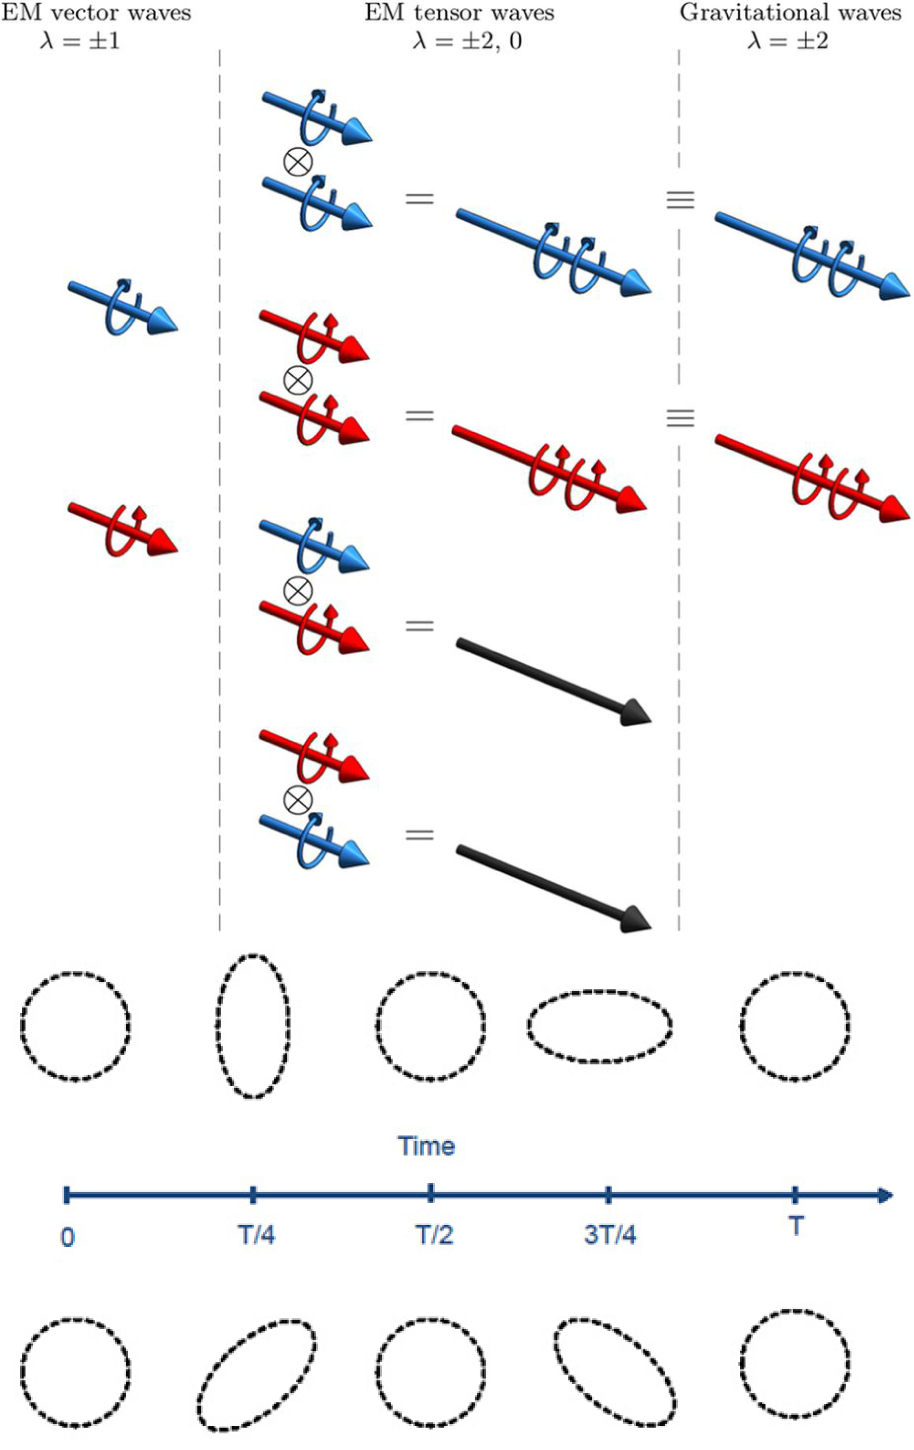
\includegraphics[width=5cm]{image/6-1-2.png}
\caption{引力波与电磁波的区别}
\end{wrapfigure}
关于场的理解历史上经历了两个过程.\,第一个阶段是正如上面的连续介质的做法,\,场是作为某种事先已经被研究的足够清楚的粒子体系与它们之间的相互作用的描述方法与数学工具.\,而从牛顿时代开始人们就默认了超距作用的存在,\,而场数学工具的第二个作用就是描述电荷之间,\,质量之间的超距作用.\,但是逐渐人们意识到相互作用传播速度的有限性,\,于是场开始变成某种与物质其他耦合的物质而单独存在,\,这就是第二阶段,\,人们意识到了场本身就是一种物质,\,电子与电子之间不能直接相互作用,\,电子改变了真空,\,稳定地与电磁场相互作用而产生库仑场,\,然后在对第二个电子产生相互作用力.\,将场作为某种先验地存在于时空中的物质形式进行描述与研究的学科就叫做\emph{场论}(field theory).\,有哪些可能的场形式?\,场的物理量如何书写?\,场与粒子,\,场与场之间如何相互作用便是场论的研究内容.\,比如说,\,动力学所关心的内容,\,场的质量本身没有定义,\,可以定义的一般是场的定域动量与波矢,\,能量与角频率,\,平面波的色散关系等等.\,的确,\,场论最基本的做法是傅里叶分解,\,它认为平面波是不受任何相互作用时的场的惯性运动方式,\,而任何场的运动,\,每一时刻都可以分解成一系列平面波的叠加.\,就好像任何复杂体系的运动本质上都是质点系的运动,\,而质点的运动每时每刻都可以看出匀速运动那样.


场论根据其描述方法分为标量场论,\,矢量场论,\,张量场论和旋量场论等.\,电磁场论是矢量场论,\,它用四势矢量$(\varphi,\bs{A})$来描述.\,引力场论在广义相对论弱场近似下是张量场论,\,但传播的引力波和电磁波类似只能有两种偏振,\,其模式为$+$型和$\times$型,\,这又是不同于电磁波的.\,在更现代的观点中,\,场是真空的某种激发,\,十分类似于一张二维的拉紧的薄膜,\,没有任何振动时它已经固有能量了,\,场物质反应为膜的各种振动形式.\,而一个石子受到外力而压弯了膜,\,就可以理解为粒子与场之间的相互作用.



\subsection{参考系,\,物理规律与其不变性}

\emph{坐标系}(coordinate system)是一套用来描述时空点位置的坐标系统,\,而\emph{参考系}(reference system)则是下文将引申的一类坐标系的统称.

在伽利略时空观\footnote{本章仅限讨论非相对论,\,相对论见后}下参考系的定义相对简单.\,我们只需要任意指定一个观察者,\,观察者可以在$3+1$维的时空中作任意运动,\,每一个时刻对应一个测量的坐标系统:\,观察者分别以右手边,\,胸前和头顶三个方向建立坐标系,\,坐标系的刻度就是其代表的位置到原点观察者处的空间距离.\,这样便可以表示任意事件的时空坐标.\,而且构成一个三维空间直角坐标系.\,叫做观察者的\emph{固有参考系}(proper reference system).

物理规律的本质是什么?\,在一个特定的参考系中,\,我们进行一些物理量的测量,\,测量得到的值之间在特定的实验条件下会满足特定的关系而不依赖于某些具体的参数,\,一般都是等式.\,这样的普遍成立的等式就可以反映某些物理规律.\,从\emph{动理学}(kinetics)的角度理解,\,体系的演化是\emph{状态}(state)随时间的演化,\,而体系的状态由一组完备的\emph{态参量}(state variable)描述,\,态参量可以包含一些广义坐标$q_\alpha$和他们对时间的导数即广义速度$v_\alpha=\dot{q}_\alpha$.\,而以下\emph{决定论}(determinism)则对物理规律的形式做出了规定:
\begin{quote}
动理学系统:

已知某时刻$t=0$的初态$\{q_\alpha(0),\,\dot{q}_\alpha(0)\}$后,\,应能预言任意将来的状态$\{q_\alpha(t),\,\dot{q}_\alpha(t)\}$.
\end{quote}

事实上,\,不光是将来的状态,\,而且在一般经典物理的框架下,\,过去的状态也是可以被``预言''的.\,这是因为我们进一步要求动理学系统的规律是以下形式的二阶方程:
\[f_i(\ddot{q}_\alpha,\,\dot{q}_\alpha,\,{q}_\alpha,\,t)=0\]

而且广义坐标的个数应该和方程的数目一致,\,方程是至多二阶的.\,微分方程的描述在数学上完全导致了体系彻底的决定性,\,只要知道初始条件便可以往前往后推理所有发生的物理现象\footnote{更有甚者,\,经典物理也难以解释耗散现象,\,在忽略耗散时,\,方程应该还具有平移对称性(不显含t)和时间反演对称性(方程对广义速度是偶函数).\,此时对将来和对过去的预言在广义速度取相反数时是完全对称的,\,而且预言只依赖与时间差不依赖于初始时刻.}.

这一物理学科研究范围内的原理很强大,\,强大到历史上很多物理学家和哲学家都质疑过它的真实性和适用性.\,最著名的莫过于拉普拉斯提出的\emph{拉普拉斯妖}(Laplace's demon)的论点:\,如果存在一个全知的拉普拉斯妖,\,能够知道在某一时刻宇宙中所有原子的精确位置与动量,\,那么任意时刻的状态也能被预言.\,这种决定论观点总是被拿来与\emph{自由意志论}(free will)去归谬,\,如果过去与未来都已经被谱写,\,那么人类所有的行为的意义和动机也就不能被解释.\,这直到今天也是科学与哲学未能获得满意的回答的问题.

但是科学的一个目的就是在于能够对未发生的事情进行预言,\,所以本着对决定论的认可与尊重,\,我们才能继续我们的科学研究.

下一个伽利略相对性原理.
\vspace{5cm}



\section{运动的描述}

\subsection{质点的运动}
质点的运动是复杂的连续体的运动的基础.\,所谓\emph{运动}(motion)就是每一个时间都有一个位置.\,就是说位置是时间的函数:
\[\bs{r}=\bs{r}(t)\]

我们使用实数上的矢量空间和矢量来刻画真实的物理学上的二维或三维空间和其中的点.\,也即:
\[\bs{r}\in\mathbb{R}^2 \;{\rm or}\; \mathbb{R}^3\]

\begin{wrapfigure}[16]{o}[-10pt]{7cm}\label{6-1-3}
\vspace{-0.4cm}
\centering
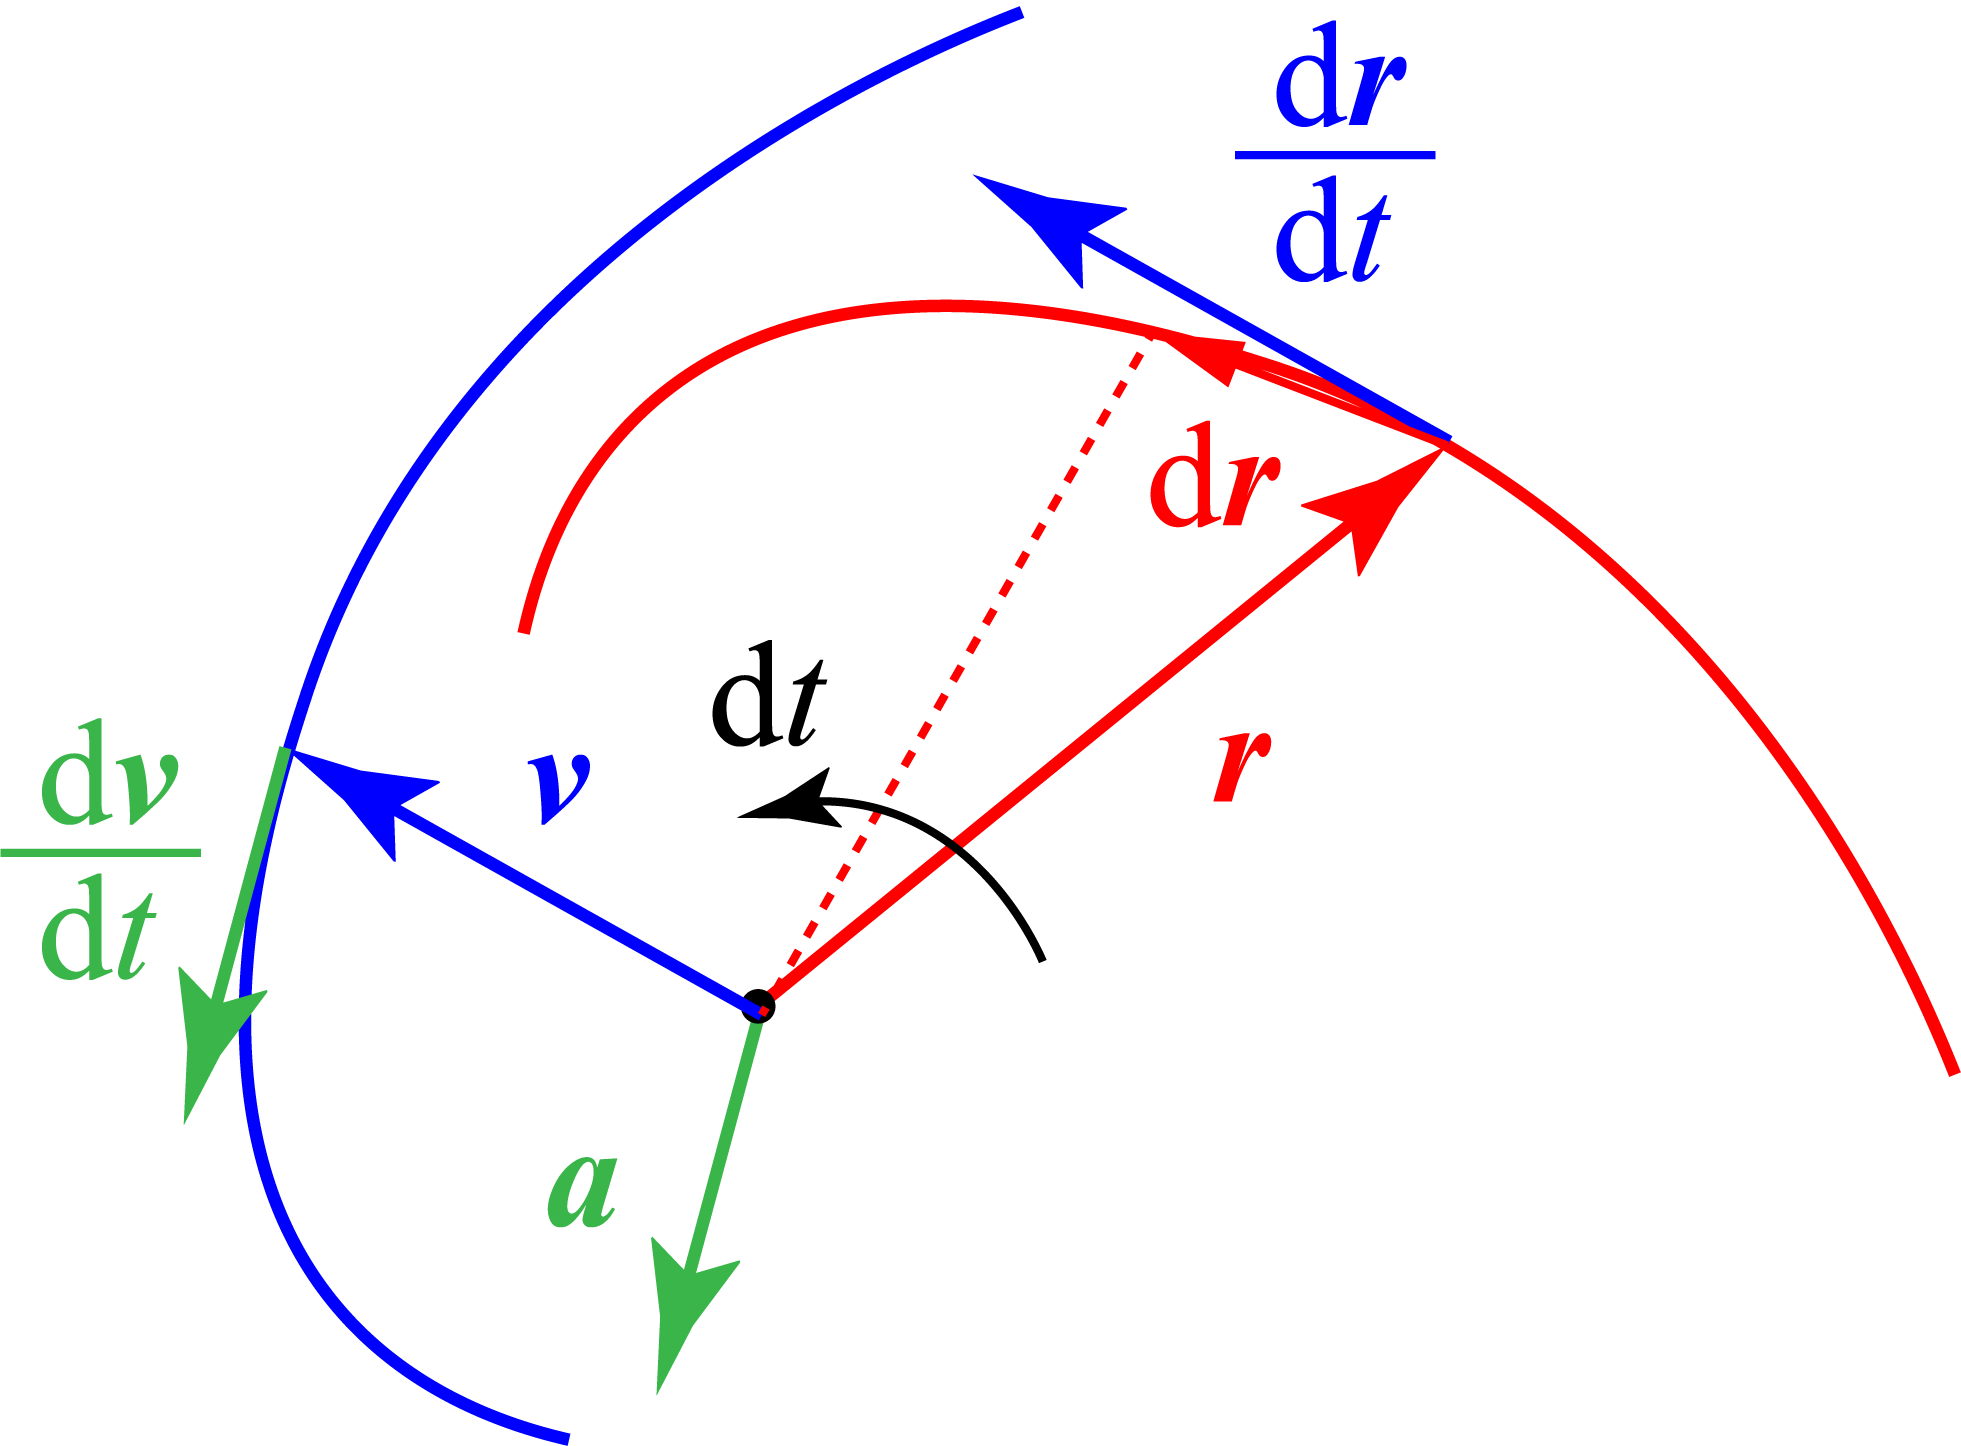
\includegraphics[width=7cm]{image/6-1-3.png}
\caption{质点的位置,\,速度与加速度}
\end{wrapfigure}
前者对应二维运动,\,后者对应三维运动.\,我们从中可以发现,\,函数是描述运动的数学工具,\,对矢量与函数的分析学知识便是运动学和物理学的基础.\,而运动学本身是可以看成是数学的一个分支的.\,对质点的位置矢量求导数便得到速度矢量,\,再求导数或是求二阶导数便是加速度矢量:
\[\bs{v}=\frac{\ud \bs{r}}{\ud t}=\lim_{\Delta t\to 0 }\frac{\bs{r}(t+\Delta t)-\bs{r}(t)}{\Delta t}\]
\[\bs{a}=\frac{\ud \bs{v}}{\ud t}=\lim_{\Delta t\to 0 }\frac{\bs{v}(t+\Delta t)-\bs{v}(t)}{\Delta t}\]
\[\bs{a}=\frac{\ud ^2\bs{r}}{\ud t^2}=\lim_{\Delta t\to 0 }\frac{[\bs{r}(t+\Delta t)-\bs{r}(t)]-[\bs{r}(t)-\bs{r}(t-\Delta t)]}{\Delta t^2}\]

正如上图\ref{6-1-3}所示,\,我们可以把每一个瞬时的速度矢量共起点画出来,\,并把端点连做曲线,\,此时背景的空间往往叫做\emph{速度空间}(velocity space),\,它的更普遍的对应是动量空间,\,这在近代物理的理论值具有重要地位.\,引入速度空间后质点的运动便可以等价地在速度空间中进行研究.\,比如在均匀重力场中的抛体运动在速度空间中就是简单的竖直向下的匀速直线运动.\,而平方反比力下的天体运动(开普勒问题)实际上在速度空间中可以证明将变为变速偏心圆周运动.\,这使得通过速度求加速度就好像通过位置求速度那样方便.\,具体求法接下来还得进一步展开.

加速度的导数偶尔也会进入物理研究的视野,\,它被叫做\emph{急动度}(jerk).\,即:
\[\bs{j}=\frac{\ud \bs{a}}{\ud t}=\frac{\ud ^3\bs{r}}{\ud t^3}\]

矢量函数概念就是实数到矢量的映射,\,但是具体能写出函数形式的例子在物理中却不是那么常见.\,比如抛体运动的运动对应的函数,\,即\emph{运动方程}(equation of motion)\footnote{指运动学运动方程,\,动力学运动方程就是反应运动的规律的,\,能够最终解出来运动学运动方程的微分方程.}为:
\[\bs{r}=\bs{r}_0+\bs{v}_0 t+\frac{1}{2}\bs{g}t^2\]

它是牛顿定律下以下微分方程结论的解:
\[\bs{a}=\frac{\ud ^2\bs{r}}{\ud t^2}=\bs{g}\]

但是在一般情况下,\,要表示出一个既有大小又有方向的矢量函数,\,我们得采用分解的思想,\,研究能够完全确定这个矢量值的参数.\,通常有以下做法:

\vspace{0.2cm}
{\bf 1.\,直角坐标系下的分解}

在一个欧几里得空间里的一个参考系中研究问题,\,很常见的一种做法是建立直角坐标系来表示一个点的位置.\,以更普遍的三维运动为例.\,既然物体的位置由坐标$(x,\,y,\,z)$来表示.\,我们就能认为表示运动的任务由三个标量函数$x(t),\,y(t),\,z(t)$来承担.\,其实这与上面介绍的用矢量来表示位置是非常一致的,\,因为实际上点的坐标通常也被理解为原点指向这个点的矢量在三个基矢的坐标:
\[\bs{r}=(x,\,y,\,z)=x\bs{i}+y\bs{j}+z\bs{k}\]

出于哈密顿(Hamilton)爵士关于把三维空间三个方向基矢视作四元数代数运算的旋转等效的奇妙观点,\,我们分别把$x,\,y,\,z$方向的基矢按照惯例记做$\bs{i},\,\bs{j},\,\bs{k}$.\,也常常因为它们是单位矢量(长度为1),\,而记做$\bs{e}_x,\,\bs{e}_y,\,\bs{e}_z$.\,这样便能把$\bs{r}$分解出$x$,\,$y$,\,$z$来.

分解以后,\,重新合成便能得到需要的物理量.\,这其中的意思是:\,比如我们为了求一个曲线运动速度或者加速度的$x$分量.\,也就是求下列表达式:
\[\bs{v}=v_x\bs{i}+v_y\bs{j}+v_x\bs{k}=\frac{\ud \bs{r}}{\ud t}\]
\[\bs{a}=a_x\bs{i}+a_y\bs{j}+a_x\bs{k}=\frac{\ud^2 \bs{r}}{\ud t^2}\]

中的分量$v_x,\,a_x$.\,其求法非常直接,\,便是:
\[v_x=\frac{\ud }{\ud t}x(t)\quad,\quad a_x=\frac{\ud^2 }{\ud t^2}x(t)\]

这相当于是说,\,求导数和向某固定方向投影是可以交换前后次序的:

\[\bs{i}\cdot \frac{\ud }{\ud t}\bs{r}=\frac{\ud }{\ud t}(\bs{i}\cdot \bs{r})\quad,\quad \bs{i}\cdot \frac{\ud }{\ud t}\bs{v}=\frac{\ud }{\ud t}(\bs{i}\cdot \bs{v})\]

这是当然的,\,因为矢量点乘的导数的法则也符合与标量乘积求导数类似的莱布尼茨法则,\,而常矢量$\bs{i}$不随着运动改变.\,所以导数只有对$\bs{r},\,\bs{v}$求导的项.

在数学上,\,曲线段也经常被描述为是与某实数上区间\emph{同胚}(homeomorphic)的几何图形,\,这其实就是说,\,存在自变量$t$,\,不失一般性地,\,我们让其取值范围为$(-\infty,\,+\infty)$.\,而存在一个从这个自变量到三维空间点$(x,\,y,\,z)$的光滑映射:
\[x=x(t)\quad ,\quad y=y(t)\quad ,\quad z=z(t)\]

\begin{wrapfigure}[10]{o}[-10pt]{7cm}\label{6-1-4}
\vspace{-0.4cm}
\centering
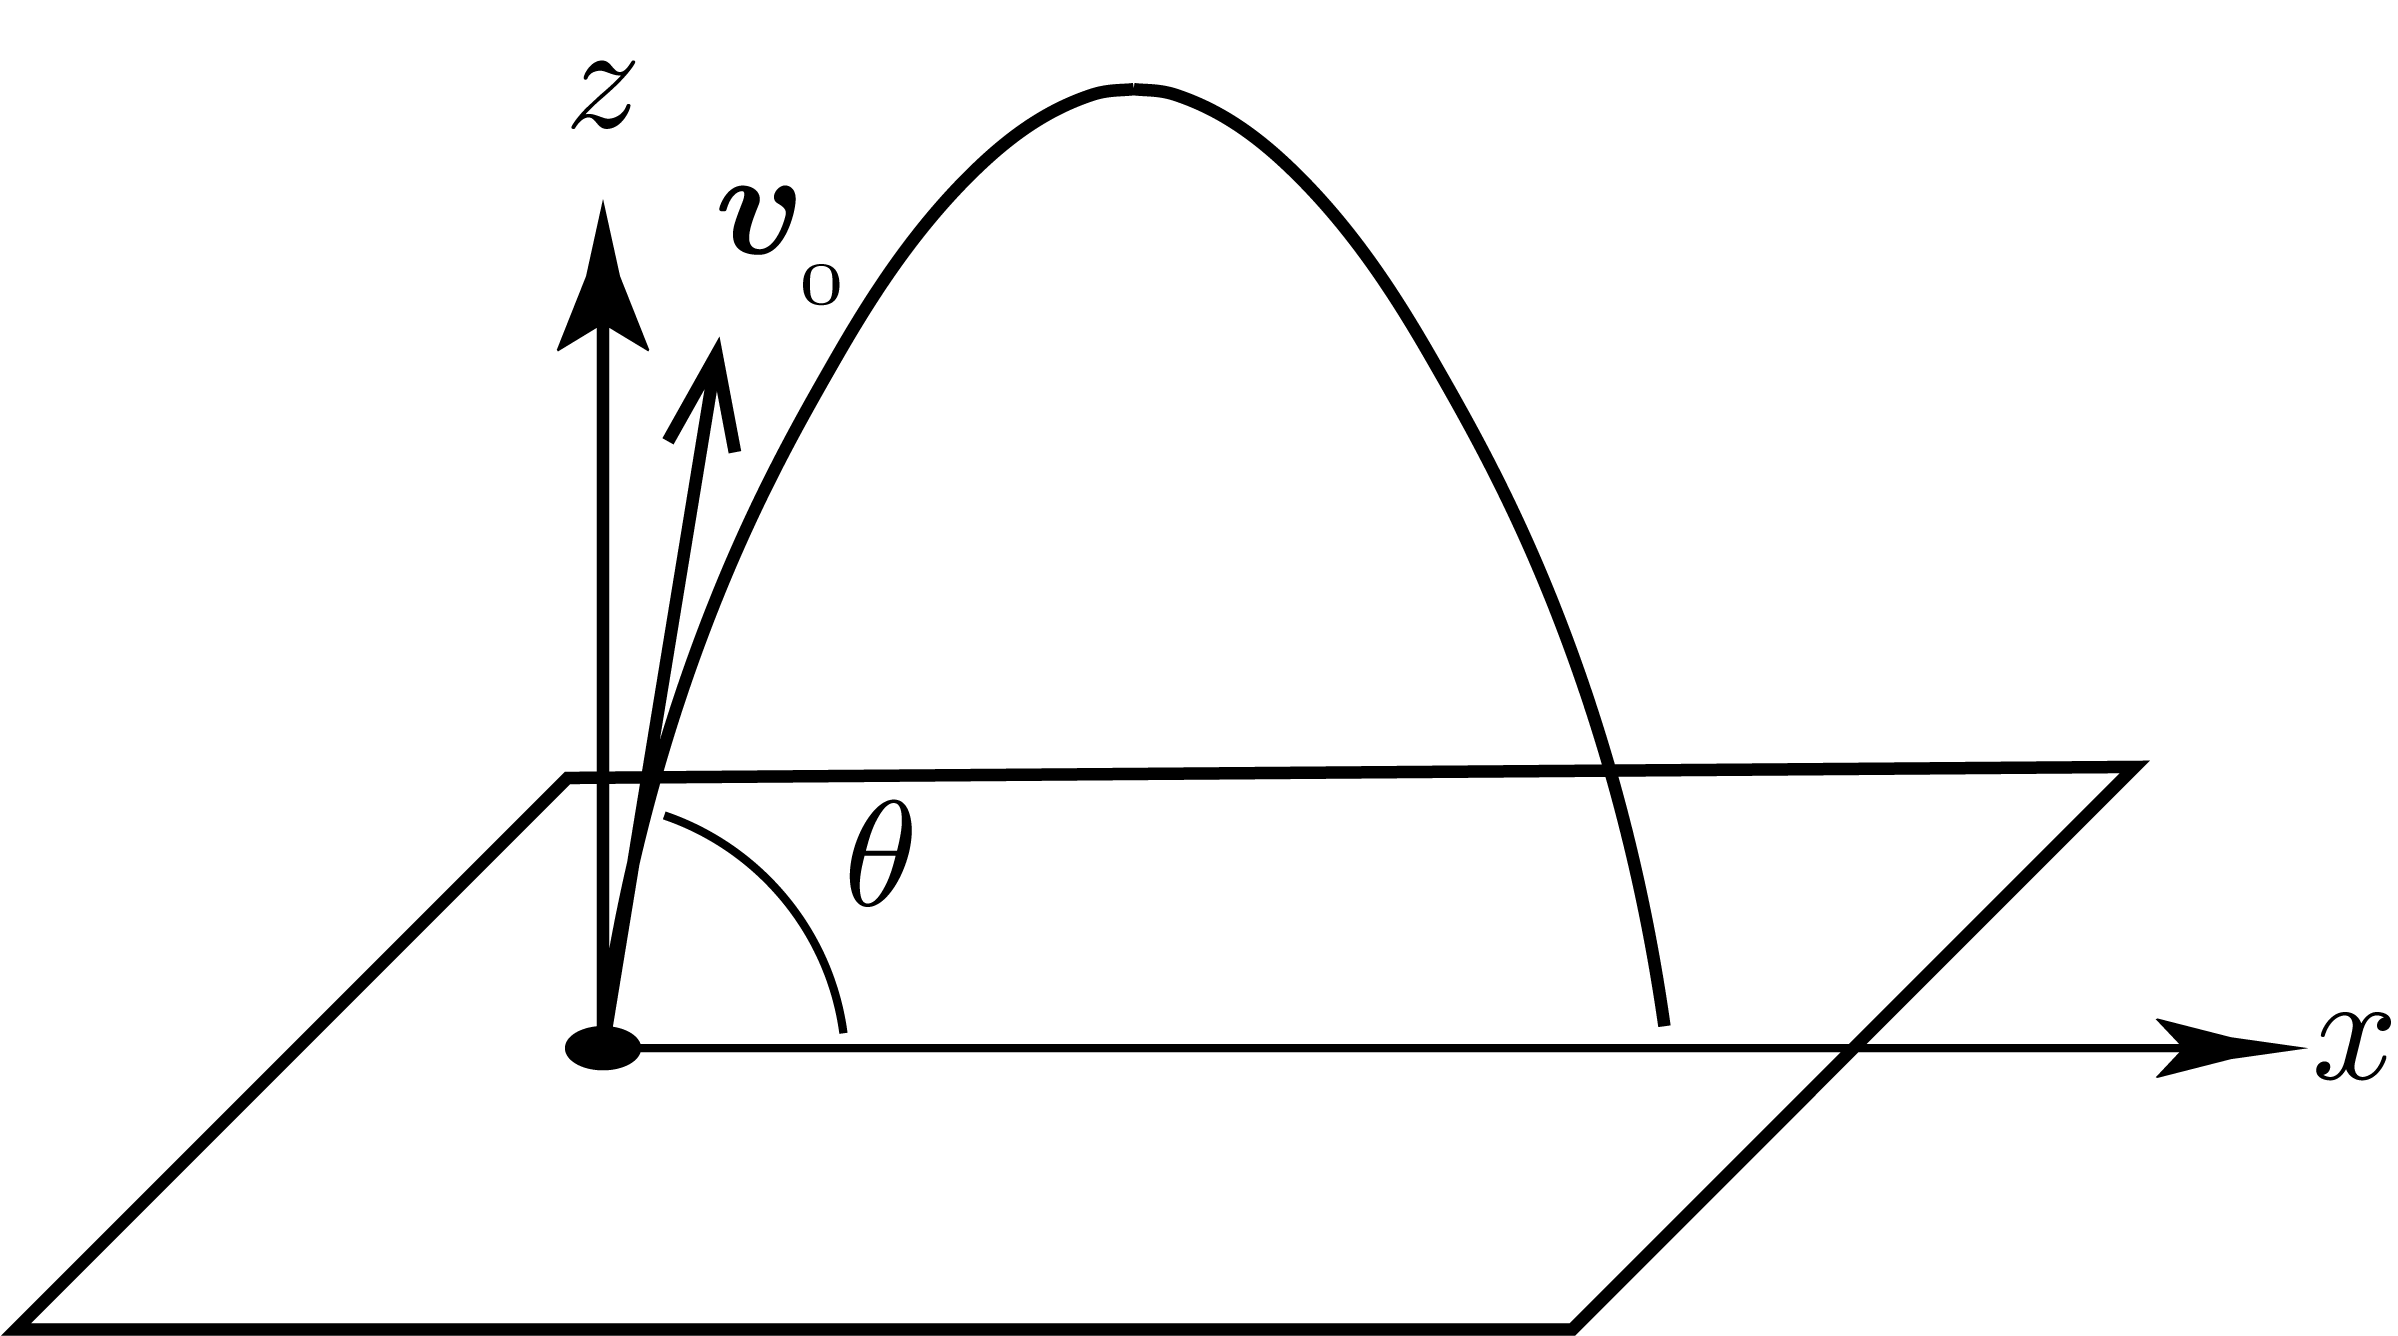
\includegraphics[width=7cm]{image/6-1-4.png}
\caption{抛体运动}
\end{wrapfigure}
在数学上看,\,这其实就是曲线方程:\,其参数方程的唯一给法.\,这样的式子就给出了几何学上的光滑曲线的定义.\,而不同于以往我们对曲线是$y=f(x)$的图像的刻板认识.\,但在这里,\,我们恰巧发现如果把参数$t$理解为时间的话,\,这恰好就对应到了一个粒子在三维空间中的运动,\,出于这样的原因,\,我们把反应了粒子位置随着时间变化的方程称为运动方程.\,它是\emph{轨迹方程}(function of trajactory)的一种特殊情况.\,对于轨迹方程,\,我们只需要通过符合方程的点$(x,\,y,\,z)$构成粒子所有运动中经过的位置构成的集合即可.\,例如,\,在地面$z=0$出发以仰角$\varphi$斜抛一个物体.\,那就以出发点为原点建立坐标系,\,竖直向上为$z$轴,\,抛的方向向前为$x$轴.\,那么运动方程为:
\[\left\{\begin{array}{l} x=v_0 t\cos\varphi\\ z=v_0 t\sin\varphi - \dfrac{1}{2}gt^2\end{array}\right.\]

但是轨迹方程不仅可以写成以上形式,\,还可以消去$t$得到:
\[z=x\tan\varphi -\frac{gx^2}{2v_0^2}(1+\tan^2\varphi)\]

\vspace{0.2cm}
{\bf 2.\,平面极坐标系下的分解}

如果质点做平面运动,\,那么我们问题得到了简化.\,此时往往有些情形下我们关心从原点的观察者出发看质点的运动时,\,质点离观察者的距离和质点相对观察者的方位.\,故引入\emph{极坐标系}(polar coordinate system)是自然而然的做法.\,其步骤为:\,确定观察者位置为\emph{极点}(pole),\,引出一条原点出发的射线为\emph{极轴}(polar axis);\,测量质点位置到极点距离$r$为\emph{矢径}(radius);\,从极点指向质点位置形成矢量矢径$\bs{r}$,\,测量极轴绕极点沿指定的正方向旋转到与矢径重合时旋转的角度$\theta$为\emph{极角}(polar angle).\,描述质点的位置时,\,$(r,\,\theta)$即构成极坐标.

仍然,\,极坐标可以用来表示质点的唯一位置:\,只需要给出$(r,\,\theta)$就可以确定位置.\,所以只要知道函数$r(t),\,\theta(t)$就能够确定其运动,\,这便是极坐标下的运动方程.\,同理如果消去$t$就能得到另一类轨迹方程.\,只要物体运动轨迹不经过极点,\,我们总是取$r(t),\,\theta(t)$为光滑的函数.\,$\theta$的取值为$(-\infty,\,+\infty)$以保证运动的连续性.\,不过$\theta$相差$2k\pi,\,k\in\mathbb{Z}$的所有坐标表示运动过程中的同一位置.

例如,\,在之前的抛体运动中,\,如果取$z$轴为极轴,\,那么其极坐标下的运动方程为:
\[\left\{\begin{array}{l} r^2=(\bs{v}_0 t+\dfrac{1}{2}\bs{g}t^2)^2=\dfrac{1}{4}g^2t^4  -gv_0t^3\sin\varphi + v_0^2t^2\\[3pt] \tan\theta=\dfrac{2v_0 \cos\varphi}{2v_0 \sin\varphi-gt}\end{array}\right.\]

这会有利于我们分析一些问题.\,例如如果关心以何种倾角抛出一个物体,\,物体离我们的距离会越来越远?\,就只需要让$r$为关于$t$的增函数,\,除了对$r$求导的做法,\,一种更加明智的做法可能是注意到关系式:
\[\frac{\ud r}{\ud t}>0  \quad\Leftrightarrow\quad	\frac{\ud}{\ud t}(\frac{1}{2}r^2)>0\]
\begin{align*} 
\Leftrightarrow \frac{\ud}{\ud t}(\frac{1}{2}r^2)	&=\frac{\ud}{\ud t}(\frac{1}{2}{\bs{r}\cdot\bs{r}})=\bs{r}\cdot\bs{v}\\
																			&=(\bs{v}_0 t+\dfrac{1}{2}\bs{g}t^2)\cdot(\bs{v}_0 +\bs{g}t)>0\\
\end{align*}

\[\Leftrightarrow (\bs{v}_0 +\dfrac{1}{2}\bs{g}t)\cdot(\bs{v}_0 +\bs{g}t)=\dfrac{1}{2}g^2t^2  -\dfrac{3}{2}gv_0t\sin\varphi + v_0^2>0\]

这就化为求关于$t$的二次函数恒大于零的系数条件问题,\,结论是初等的:\,判别式小于零:
\[\left(\dfrac{3}{2}gv_0\sin\varphi\right)^2-4\left(\dfrac{1}{2}g^2 \right)(v_0^2)<0\quad \Rightarrow\quad \sin\varphi<\frac{2\sqrt{2}}{3}\]

采用极坐标系描述抛体运动也许是费力而不讨好的.\,但是描述其他一些运动又比直角坐标系存在天然的优势.\,比如一类经典问题的表述如下:\,



\section{参考系变换}

\section{运动的牵连}

